\chapter{Modellare le Operazioni}
Per operazione intendiamo cosa fa il sistema per raggiungere i goal e 
come vengono rappresentate le operazioni.

Le operazioni riguardano le \textbf{operazioni attive}, ovvero le azioni
che il sistema deve compiere per raggiungere i goal.

\section{Operation model}
Si tratta di una vista \textbf{funzionale del sistema} che rappresenta \textbf{quali} 
servizi saranno resi disponibili all'interno del sistema e \textbf{sotto quali 
condizioni} per il soddisfacimento dei goal.

La rappresentazione avviene sempre mediante l'ausilio dei diagrammi \texttt{UML}
declinati ina maniera funzionale alla modellazione dei requisiti.

Gli obiettivi di tale diagramma sono molteplici, tra cui:
\begin{itemize}
    \item Fornire un input agli sviluppatori per la specifica del software.
    \item Descrivere le procedure e i task all'interno dell'ambiente.
    \item Può essere un punto di partenza per identificare con quali dati 
    interagirà il sistema o essere l'input per i tool di prototipazione o 
    animazione dei requisiti.
    \item Possiamo utilizzarli per stimare i \textit{function point}, ovvero 
    capire quanto lavoro ci sarà da fare per l'implementazione delle varie 
    componenti.
    \item Permette di creare un link tra tutte le funzionalità del sistema e 
    i goal che si vogliono raggiungere.
\end{itemize}

\section{Le operazioni}
\begin{tcolorbox}[colback=violet!5!white,colframe=violet!75!black, title=Operazione]
    Una \textbf{operazione} è una coppia di stati del sistema, di \textit{input} e 
    \textit{output}. Un'operazione ci permette di cambiare lo stato del sistema.
\end{tcolorbox}
Ricordiamo che uno stato è una tupla $x_i \rightarrow v_i$, dove $x_i$ rappresenta 
l'attributo di una istanza di oggetto concettuale, mentre $v_i$ rappresenta il valore che 
assume tale attributo.

Abbiamo diverse tipologie di variabili coinvolte nelle operazioni:
\begin{itemize}
    \item Variabili di \textbf{input}: rappresentano i dati che il sistema riceve in
    input per poter eseguire un'operazione.
    \item Variabili di \textbf{output}: rappresentano i dati che il sistema restituisce
    in output dopo aver eseguito un'operazione.
\end{itemize}

Anche le operazioni possono avere \textbf{attributi} che ne specificano le
caratteristiche.

\subsubsection{Esempio}
Consideriamo l'operazione \textit{OpenDoors(tr)}, lo stato iniziale del 
sistema è 
\[(tr.Speed \rightarrow 0, tr.DoorState \rightarrow 'Closed')\]

mentre lo stato finale diventa:

\[(tr.Speed \rightarrow 0, tr.DoorState \rightarrow 'Open')\]

\begin{tcolorbox}
    L'obiettivo è di \textbf{operazionalizzare} i goal del goal model, ovvero
    permettere in maniera operativa di raggiungere i goal.
\end{tcolorbox}

Le operazioni sono:
\begin{itemize}
    \item \textbf{Deterministiche}: non hanno quindi un comportamento
    probabilistico.
    \item \textbf{Atomiche}: non possono essere suddivise in operazioni più
    piccole. 
    \item \textbf{Possono essere applicate in modo parallelo}: possono essere
    eseguite in modo parallelo.
\end{itemize}

\section{Rappresentare le operazioni}
Le operazioni vengono rappresentate mediate l'ellisse come nel \textbf{Use Case Diagram}.

\begin{figure}[H]
    \centering
    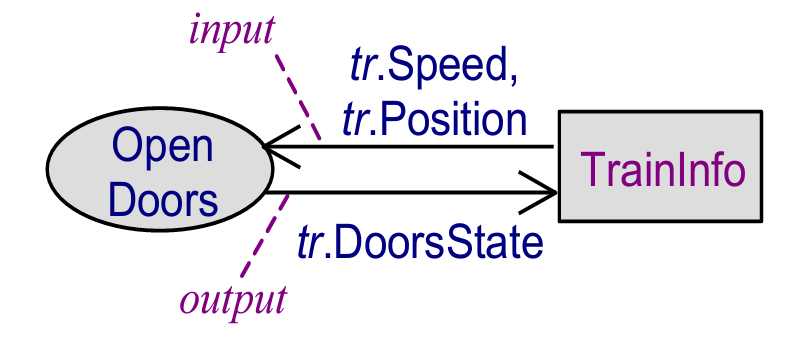
\includegraphics[scale = 0.3]{img/operation.png}
    \caption{Rappresentazione di un'operazione}
\end{figure}
Potrebbero avere anche delle precondizioni e delle postcondizioni, all'interno di un 
commento \texttt{UML}, insieme a \textbf{input} e \textbf{output}.
\subsubsection{Esempio}
\begin{itemize}
    \item \textbf{Operation}: TrainInfo
    \item \textbf{Input}: tr: TrainInfo / \{Speed, Position\}
    \item \textbf{Output}: tr: TrainInfo / \{DoorState\}
\end{itemize}
\subsection{Pre e post condizioni di Dominio}
\begin{tcolorbox}[colback=yellow!5!white,colframe=yellow!75!black, title=Precondizioni]
    Le \textbf{precondizioni} sono le condizioni che devono essere verificate
    affinché l'operazione possa essere eseguita.
\end{tcolorbox}
\begin{tcolorbox}[colback=orange!5!white,colframe=orange!75!black, title=Postcondizioni]
    Le \textbf{postcondizioni} sono le condizioni che devono essere verificate
    affinché l'operazione sia stata eseguita correttamente.
\end{tcolorbox}
Rispettivamente vengono descritte con \textbf{DomPre} e \textbf{DomPost}. Entrambe sono 
degli statement \textbf{descrittivi}. 
\subsection{Esecuzione di un'operazione}
Sostanzialmente il link tra le operazioni e gli agenti è un link di \textbf{performing}.
\begin{tcolorbox}
    Gli agenti attuano le operazioni per raggiungere i goal di cui è responsabile.
\end{tcolorbox}
Ci sono delle regole di consistenza che devono però essere rispettare:
\begin{itemize}
    \item Le variabili di input e output devono essere grandezze \textit{monitorabili}
    e \textit{controllabili} dagli agenti.
    \item Ogni operazione può essere intrapresa da un solo agente (\textit{problematiche 
    di responsabilità}).
\end{itemize}
\section{Operalizzazione dei goal}
La metodologia goal oriented permette di \textbf{operazionalizzare} i leaf goal, e questo 
è il motivo primario per cui abbiamo la destrutturazione dei goal di alto livello in goal
di basso livello.
\subsection{Condizioni Pre, Post, Trigger per il soddisfacimento dei goal}
Abbiamo un link di operalizzazione che collega un'operazione a un requisito (\textit{leaf goal}).
Anche in questo caso tale link può avere degli attributi, tra cui:
\begin{itemize}
    \item \textbf{ReqPre}: le condizioni \textit{necessarie} affinché l'operazione possa
    soddisfare il goal (\textbf{deve}).
    \item \textbf{ReqTrig}: le condizioni \textit{sufficienti} affinché l'operazione possa
    soddisfare il goal (\textbf{può}).
    \item \textbf{ReqPost}: le condizioni che devono essere verificate affinché l'operazione
    abbia soddisfatto il goal.
\end{itemize}

\subsubsection{Esempio completo}
\begin{itemize}
    \item \textbf{Operazione}: OpenDoors
    \begin{itemize}
        \item \textbf{Def}: Operazione che controlla l'apertura di tutte le porte
        di un treno.
        \item \textbf{Input}: \texttt{tr}: TrainInfo / \{Speed, Position\}
        \item \textbf{Output}: \texttt{tr}: TrainInfo / \{DoorState\}
        \item \textbf{DomPre}: Le porte del treno \texttt{tr} sono chiuse.
        \item \textbf{DomPost}: Le porte del treno \texttt{tr} sono aperte.
        \item \textbf{ReqPre}: Il velocità del treni \texttt{tr} è zero.
        \item \textbf{ReqPre}: il treno \texttt{tr} è in stazione.
        \item \textbf{ReqTrig}: Il treno \texttt{tr} si è appena fermato in stazione.
    \end{itemize}
\end{itemize}

\begin{tcolorbox}
    Generalmente un leaf goal è operazionalizzato da più operazioni, e delle operazioni possono
    operazionalizzare più leaf goal.
\end{tcolorbox}
Quando succede, tutte le precondizioni e le postcondizioni devono essere implicitamente
congiunte.
Se una precondizione di dominio è vera, deve essere applicata appena la condizione di trigger 
diventa vera. Se una precondizione di dominio può essere applicata quando 
tutte le condizioni di operalizzazione sono vere.

\begin{tcolorbox}[title=Consistenza]
    Se una precondizione di dominio è vera e almeno una delle condizioni di trigger 
    è vera, allora tutte le preconditioni di operalizzazione devono essere vere.
\end{tcolorbox}

\subsection{Impegno degli agenti}
Per ogni goal sotto la responsabilità di un agente, e per ogni operazione che 
operalizza un goal, abbiamo che l'agente deve garantire che l'operazione sia 
applicata quando:
\begin{itemize}
    \item Quando le operazioni \textbf{DomPre} sono vere.
    \item Appena le operazioni \textbf{ReqTrig} diventano vere.
    \item Solo se le operazioni \textbf{ReqPre} sono vere.
    \item In Modo tale che le operazioni \textbf{DomPost} e \textbf{ReqPost} siano vere.
\end{itemize}
Di fronte agli agenti ci troviamo di fronte a un \textbf{non determinismo}, poiché potremmo 
trovarci di fronte a due categorie di agenti:
\begin{itemize}
    \item \textbf{Eager}: l'agente fa partire l'operazione non appena
    le condizioni \textbf{ReqPre} sono vere.
    \item \textbf{Lazy}: l'agente aspetta che le condizioni \textbf{ReqTrig}
    siano vere, quando si trova costretto.
\end{itemize}
Ci troviamo quindi di fronte a un certo grado di libertà per gli agenti, che
possono decidere quando far partire le operazioni e una sorta di concorrenza
tra le gli agenti stessi.
\subsection{Operalizzazione dei goal e soddisfacimento}
Consideriamo l'operalizzazione di un goal in concomitanza con la soddisfacibilità
dei goal, l'operation model e il goal model possono argomentare sugli obiettivi di 
alto livello che vengono raggiunti.
Di fatto possono essere percorsi:
\begin{itemize}
    \item All'indietro: capire perché un goal è stato raggiunto.
    \item In avanti: capire come un goal può essere raggiunto.
\end{itemize}
\section{Rappresentazione semantica}
\begin{figure}[H]
    \centering
    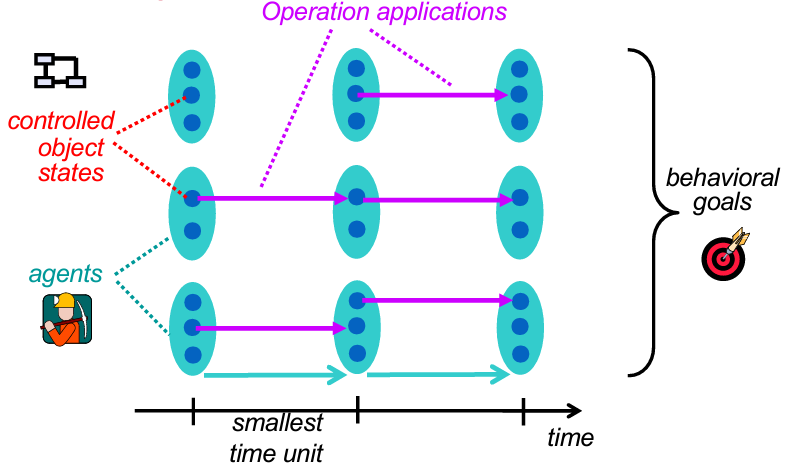
\includegraphics[scale = 0.3]{img/operalizzazione.png}
    \caption{Rappresentazione semantica delle operazioni}
\end{figure}
Le operazioni si applicano nel corso del tempo attuano cambiamenti 
di stato all'interno del sistema, controllando lo stato degli oggetti.
\subsection{Use Case Diagram}
Nel tempo possono non far nulla o modificare lo stato di uno o più agenti 
che può controllare. 

Le operazioni possono essere rappresentati mediante \textbf{use case diagram} rappresentando
le operazioni e gli agenti.

Ho delle interazioni con:
\begin{itemize}
    \item L'agente che controlla le operazioni in input 
    \item L'agente che monitora operazioni in output
\end{itemize}
Ci sono dei link tra le operazioni di \textbf{extend} e \textbf{include}.
\begin{itemize}
    \item \textbf{Include}: l'operazione include un'altra operazione.
    \item \textbf{Extend}: l'operazione estende un'altra operazione.
\end{itemize}
Dobbiamo però ricordarci che le operazioni sono atomiche, non decomponibili in 
sotto operazioni, perciò questa tipologia di link non sarebbe da utilizzare.

\subsubsection{Esempio}
\begin{figure}[H]
    \centering
    \begin{tikzpicture}
        % Definizione del sistema
        \begin{umlsystem}[x=4, fill=red!10]{OnBoardController}
          \umlusecase[x=3, y=-1]{SendAccelerationCommand}
          \umlusecase[x=3, y=-2]{OpenDoors}
          \umlusecase[x=3, y=-3]{CloseDoors}
        \end{umlsystem}
      
        % Definizione degli attori
        \umlactor[x=0, y=-1.25]{SpeedSensorAndAccelController}
        \umlactor[x=0, y=-3.25]{doorsActuator}
    
        % Associazioni 
        \umlassoc{SpeedSensorAndAccelController}{usecase-1}
        \umlassoc{doorsActuator}{usecase-2}
        \umlassoc{doorsActuator}{usecase-3}
    \end{tikzpicture}
    \caption{Rappresentazione semantica delle operazioni}
\end{figure}
\section{Derivare operazioni dai goal in maniera fluida}
\begin{itemize}
    \item La prima modalità consiste nell'utilizzare i \textit{fluents},
    i fluents non sono altro che condizioni che definiscono l'avvio o il 
    termine di una qualche operazione.
    Consideriamo \textit{Le porte del treno sono chiuse se il treno è in movimento}.
    In questo caso distinguiamo $\texttt{Moving} \rightarrow \texttt{Closed}$.
    \item Possiamo utilizzare le interazioni all'interno degli scenari. Gli 
    scenari possono essere metodologie per l'espressione dei requisiti.
    \begin{figure}[H]
        \centering
        \begin{tikzpicture}
            \begin{umlseqdiag}
              % Definizione degli oggetti
              \umlactor[class=Initiator, x=0]{in}
              \umlobject[class=Scheduler, x=4]{s}
              \umlobject[class=Participant, x=8]{p}
          
              % Messaggi
              \begin{umlcall}[op=meetingReq(dateRange), type=synchron]{in}{s}
              \end{umlcall}
              
              \begin{umlcall}[op=OK-request, type=synchron, return=]{s}{in}
              \end{umlcall}
              
              \begin{umlcall}[op=? constraints, type=synchron, return=]{s}{p}
              \end{umlcall}
              
              \begin{umlcall}[op=! constraints, type=synchron, return=]{p}{s}
              \end{umlcall}
              
              \begin{umlcall}[op=OK-constr, type=synchron, return=]{s}{in}
              \end{umlcall}
              
              \begin{umlcall}[op=scheduleSetting, type=synchron, return=]{s}{p}
              \end{umlcall}
              
              \begin{umlcall}[op=notification(date), type=synchron, return=]{p}{s}
              \end{umlcall}
              
              \begin{umlcall}[op=notification(date), type=synchron, return=]{s}{in}
              \end{umlcall}
            \end{umlseqdiag}
          \end{tikzpicture}
    \end{figure}
    \item Rafforzamento delle precondizioni e postcondizioni con condizioni
    richieste dagli obiettivi
    \begin{itemize}
        \item \textbf{Identificare i permessi richiesti}: se l'effetto DomPost di un'operazione può violare un obiettivo \( G \) sotto condizione \( C \)
        \begin{itemize}
            \item \texttt{ReqPre per \( G \)}: \texttt{non \( C \)}
            \item \textbf{es.} OpenDoors: \texttt{ReqPre per "Moving \(\rightarrow\) Closed"}: \texttt{non Moving}
        \end{itemize}
    
        \item \textbf{Identificare le obbligazioni richieste}: se l'effetto DomPost
        di un'operazione è prescritto da un obiettivo \( G \) da mantenere ogni volta che la condizione \( C \) diventa \texttt{true}
        \begin{itemize}
            \item \texttt{ReqTrig per \( G \)}: \texttt{\( C \)}
            \item \textbf{es.} OpenDoors: \texttt{ReqTrig per "StoppedAtPlatform
            \(\rightarrow\) Open"}: \\\texttt{StoppedAtPlatform}
        \end{itemize}
    
        \item \textbf{Identificare gli effetti aggiuntivi richiesti}: se il
        DomPost di un'operazione non è sufficiente per garantire la condizione
        target \( T \) di un obiettivo \( G \)
        \begin{itemize}
            \item \texttt{ReqPost per \( G \)}: \texttt{condizione mancante da \( T \)}
            \item \textbf{es.} PlanMeeting: \texttt{ReqPost per ConvenientMeeting}:
            \\\texttt{data non in date escluse}
        \end{itemize}
    \end{itemize}
\end{itemize}


  